\section{\gls{lusc} Clinical and Molecular Context}

\subsection{Epidemiology and Clinical Significance}

%TODO:checkif this data is accurate and uptodate; and add sources

Lung cancer is the leading cause of cancer-related deaths worldwide, accounting for an estimated 2.5 million new cases and 1.8 million deaths in 2020; more than the combined mortality of colorectal, breast, and prostate cancers \parencite{Bray2024}. Despite representing approximately 12\% of all new cancer diagnoses, lung cancer is responsible for nearly 18\% of all cancer deaths. This disparity reflects the severity of lung cancer, reflecting late-stage presentation, aggressive biology, and narrow actionable-driver landscape in its most common histological subtype, \gls{lusc} \parencite{Bray2024, Sung2021}. 

%TODO: add a figure here showing subtypes of lung cancer; luad and lusc; and include source

Clinically, lung cancers are stratified into two major categories: \gls{sclc}, which accounts for 13-15\% of all cases, and is characterised by rapid proliferation, early metastasis, and initial but transient chemosensitivity \parencite{Herbst2018}, and \gls{nsclc} which comprises the remaining 85\% and is itself heterogeneous. Within \gls{nsclc}, the major histological subtypes are \gls{luad}, \gls{lusc}, and large-cell carcinoma, which together constitute majority of diagnoses. These subtypes are biologically and clinically distinct, with important implications for prognosis and treatment, molecular profiling strategy, and therefore the design of studies such as this work \parencite{Herbst2018, Mino-Kenudson2022-xp}.

% TODO: transcriptional programme? im not sure if i can call it sth else
\gls{lusc} arises preferentially in the central bronchi from squamous metaplasia of the airway epithelium following chronic carcinogen exposure, and is closely linked to tobacco use \parencite{Herbst2018, Mino-Kenudson2022-xp}. In contrast, \gls{luad} originates in peripheral lung tissue, expresses a glandular transcriptional programme, and occurs in a clinically distinct subpopulation that includes never-smokers or light-smokers at a substantially higher proportion to \gls{lusc} \parencite{Herbst2018}. Histologically, \gls{lusc} is distinguished by expression of squamous lineage markers like p40, p63 and cytokeratins CK5/6 wheres \gls{luad} expresses \gls{ttf-1} and napsin-A \parencite{Mino-Kenudson2022-xp}. These distinct tissue origins are mirrored at the molecular level: \gls{luad} is enriched for actionable alternations including \textit{EGFR} mutations (~15\% Western; ~45\% East Asian), \textit{ALK} fusions (~5\%), and \textit{ROS1}, \textit{MET}, \textit{BRAF}, and \textit{NTRK} alterations \parencite{Herbst2018}, whereas \gls{lusc} is characterised by \textit{NFE2L2}/\textit{KEAP1} pathway alterations (~30\%), \textit{SOX2} amplification (~20\%), \textit{FGFR1} amplification (~20\%), and \textit{PIK3CA} mutation (~7\%), with no approved targeted therapy for most of these alterations \parencite{Hammerman2012,Lau2022-hy}.

\gls{lusc} poses substantial clinical severity and motivates the need for improved molecular characterisation. Stage-specific five-year overall survival ranges from approximately 60-80\% at stage~I to 4-8\% at stage~IV under conventional platinum-doublet chemotherapy \parencite{Herbst2018, Lau2022-hy}. The introduction of immune checkpoint inhibitors has improved outcomes for a subset of patients: the CheckMate~017 trial demonstrated that nivolumab produced a two-year overall survival of 23\% versus 8\% with docetaxel in previously treated advanced squamous-cell \gls{nsclc} \parencite{Brahmer2015}, and the KEYNOTE-407 trial established pembrolizumab combined with platinum-based chemotherapy as a standard first-line option, yielding a median overall survival of 15.9~versus 11.3~months with chemotherapy alone \parencite{PazAres2018}. Despite these advances, outcomes for stage~IV \gls{lusc} remain substantially worse than for \gls{luad} patients with targetable drivers, who may achieve median overall survival exceeding 35~months with osimertinib
\parencite{Remon2024}. The contrast in prognosis across \gls{nsclc} subtypes and treatment eras is illustrated in Figure~\ref{fig:os_comparison}.

\begin{figure}[htbp]
    \centering
    \fbox{%
        \begin{minipage}[c][8cm][c]{0.85\textwidth}
            \centering
            \vspace{0.5cm}

            {\Large Placeholder Figure}
            \vspace{0.5cm}
        \end{minipage}
    }
    \caption{Placeholder, comparing survival outcomes across NSCLC}
    \label{fig:os_comparison}
\end{figure}

In Nepal and South Asia, lung cancer has additional public-health relevance because of tobacco use, indoor air pollution from biomass fuel combustion, outdoor air pollution from particulate matter, delayed diagnosis, and variable access to molecular diagnostics and advanced therapies \parencite{Shilpakar2022-uh, Sreeramareddy2006, Yadav2024}. Local hospital-based series show that squamous histology has historically constituted a substantial proportion of diagnosed lung cancer cases, albeit reported proportions vary by institution, time period, diagnostic method, and referral pattern (Table~\ref{tab:nepal_lung_cancer_series}). This epidemiological context further motivates the need for computational characterisation of \gls{lusc} subtypes utilising data from international cohorts, with the expectation that biologically coherent subtypes may eventually support diagnostic and prognostic applications in resource-limited settings.

%TODO: idk if top 5 or top10 would make more sense; should i keep their AQI as well? caption says compared to countries with similar AQI; so seems necessary
%also dont see source in caption

\begin{figure}[h!]
    \centering
    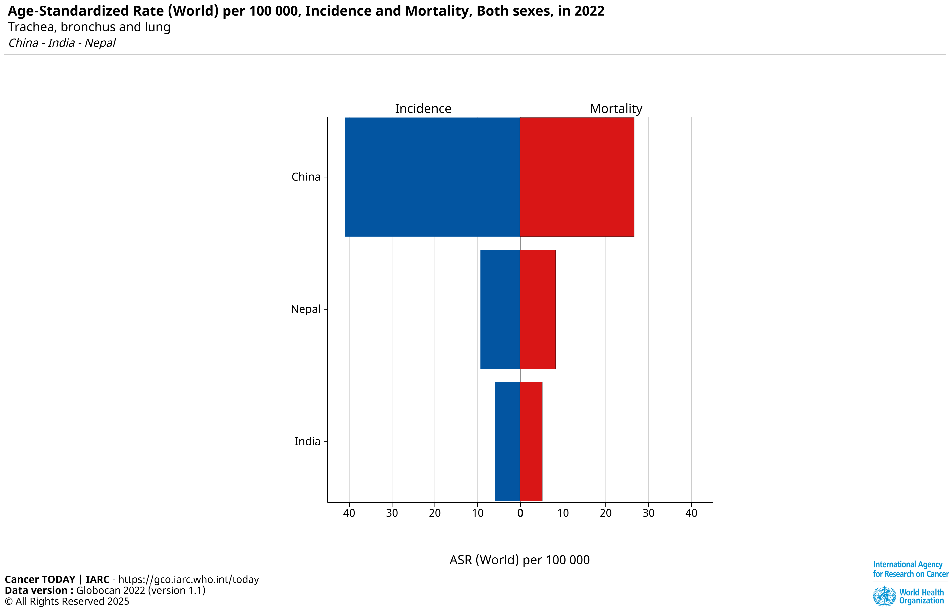
\includegraphics[width=0.75\textwidth]{figures/review/lung_cancer_asr_per_100000_2022.png}
    \caption[Trachea, bronchus and lung cancer burden in Nepal]{Incidence
    and mortality rates of trachea, bronchus and lung cancer in Nepal
    compared to countries with similar air quality profiles.}
    \label{fig:lung_cancer_burden_nepal}
\end{figure}

%TODO: check if more recent data is available from 2023-2025; did i forget to cite sources??

\begin{table}[h!]
    \small
    \caption[Lung cancer histology series in Nepal]{Selected
    hospital-based lung cancer series in Nepal reporting major
    histological categories. BPKMCH: BP Koirala Memorial Cancer
    Hospital; NCH: National Hospital and Cancer Research Center; PCH: Purbanchal Cancer Hospital.}
    \centering
    \begin{tabular}{@{}llccccp{2.2cm}@{}}
        \toprule
        \textbf{Duration} & \textbf{Study Site} & \textbf{Cases}
            & \textbf{LUSC (\%)} & \textbf{LUAD (\%)}
            & \textbf{SCLC (\%)} & \textbf{Notes} \\
        \midrule
        2001 - 2019 & BPKMCH & 250 & 72.4 & 18.4 & 1.2
            & Hospital series \\
        Jan 2000 - Dec 2009 & BPKMCH & 1074 & 33.98 & 5.21 & 13.78
            & Hospital series \\
        Sept 2001 - Aug 2005 & Case-series & 136 & 51.5 & 8.1 & 17.6
            & Case series \\
        Jan 2012 - Dec 2018 & NCH & 250 & 51.2 & 26.8 & 22.0
            & Hospital series \\
        Jan 2017 - Dec 2021 & University Hospital & 127 & 35.7 & 23.5
            & 13.3 & Hospital series \\
        Jan 2020 - Dec 2023 & PCH & 192 & 23.9
            & 33.8 & 24.5 & Hospital series \\
        \bottomrule
    \end{tabular}
    \label{tab:nepal_lung_cancer_series}
\end{table}


\subsection{Current Treatment Landscape}

Treatment of \gls{lusc} depends on stage, performance status, pathology, and biomarker profile. Early-stage disease may be managed with surgical resection, with or without adjuvant chemotherapy or chemoradiotherapy for locally advanced disease \parencite{Herbst2018, Li2023-th}. Advanced or metastatic disease is typically treated with platinum-based doublet chemotherapy, increasingly combined with immune checkpoint inhibitors \parencite{PazAres2018, Remon2024}. Unlike \gls{luad}, \gls{lusc} has a limited repertoire of actionable driver mutations, meaning that advances in precision oncology that have revolutionised \gls{luad} management for \gls{egfr}-mutation and \gls{alk}-rearranged patients remain elusive for most \gls{lusc} patients \parencite{Lau2022-hy}
%TODO: add source for this in caption; has no source at present
\begin{figure}[h!]
    \centering
    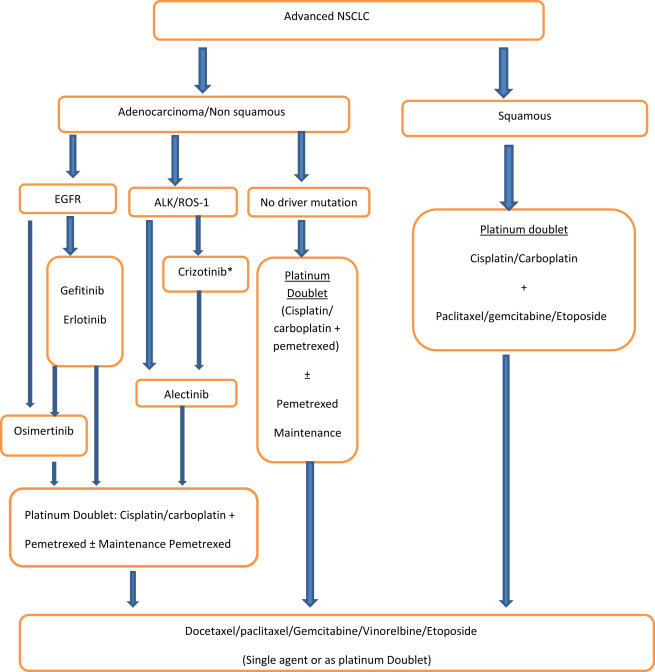
\includegraphics[width=0.8\textwidth]{figures/review/lung_cancer_treatment_approaches.png}
    \caption[Lung cancer treatment strategies]{Major treatment strategies used in lung cancer management.}
    \label{fig:lung_cancer_treatment}
\end{figure}

This therapeutic disparity in treatment of \gls{lusc} makes its molecular characterisation especially pressing. Improved subtype classification could identify biological programs like immune microenvironment composition, oxidative stress response, proliferative activity, epigenetic regulation; the spectrum of which could predict response to existing therapies or define targets for new ones. Even when subtype labels are not directly actionable, they provide a biologically interpretable framework for stratifying patients in clinical trials and for prioritising candidate biomarkers in translational research.

\subsection{Molecular Subtype Classification}

Transcriptomic studies establish \gls{lusc} not as a single molecularly uniform entity but as a collection of at least four reproducible \gls{mrna} expression subtypes. Wilkerson et al.\ described classical, basal, secretory, and primitive subtypes across five discovery cohorts and an independent validation set, using consensus clustering of gene expression profiles and nearest-centroid classifiers \parencite{Wilkerson2010}. These subtypes correspond to distinct biological programs and relate to different normal airway cell-type states, suggesting that they reflect genuine lineage and differentiation heterogeneity rather than technical artefacts \parencite{Wilkerson2010}. The \gls{tcga} characterisation subsequently validated this four-subtype taxonomy on a larger multi-platform cohort and identified subtype-specific genomic alterations, including \textit{KEAP1}/\textit{NFE2L2} alterations enriched in the classical subtype and \textit{RB1}/\textit{PTEN} alterations in the primitive subtype \parencite{Hammerman2012}.

Beyond this foundational classification, a many studies have  proposed complementary or alternative subtyping schemes  using different molecular layers and computational strategies \parencite{Bhandari2026scoping} (see Table~\ref{tab:subtyping_methods}). Proteomics-based subtyping of the CPTAC \gls{lusc} cohort revealed three subtypes associated with immune infiltration, redox activity, or mixed features, respectively, demonstrating that protein-level data captures biological axes orthogonal to transcriptomic subtyping \parencite{Stewart2019}. Methylation consensus clustering has identified up to seven epigenetic subtypes with distinct prognostic outcomes, and integration of methylation with expression data suggests that epigenetic regulation contributes independently to \gls{lusc} heterogeneity \parencite{Li2021methylation}. Immune-focused analyses have repeatedly converged on subgroups enriched in cytotoxic T cells, macrophages, or immunosuppressive regulatory programmes, with implications for checkpoint inhibitor response \parencite{Yang2022immune, Zhang2022}. More recent analyses have applied stemness indices \parencite{Lai2023stemness}, metabolic gene signatures \parencite{Ma2023metabolism, Chen2023lactate}, and tumour microenvironment deconvolution \parencite{Duan2025} to define prognostically relevant \gls{lusc} subgroups. Single-cell RNA sequencing has further resolved intratumoural heterogeneity, identifying specific macrophage and regulatory T cell subpopulations associated with prognosis \parencite{Wu2023scRNA}.
 
Collectively, these studies establish that \gls{lusc} heterogeneity is multi-layered: different molecular platforms can reveal different axes of  variation, and the subtypes identified by one platform are not always directly comparable to those identified by another. This is precisely the observation that motivates the modality-by-modality comparison in the present thesis. Rather than proposing yet another subtype system, this thesis asks which molecular layers preserve the established expression-defined subtype identity (classical, basal, secretory, primitive) most faithfully, and whether different platforms provide complementary or redundant biological information. The Wilkerson/TCGA four-subtype taxonomy is used as the reference classification because it is the most widely validated, biologically characterised, and reproducible system available \parencite{Wilkerson2010, Hammerman2012}.

%TODO: idk if all columns here are needed, and idk if there's a better way to keep sources; im not sure; and here, i want to cite my own preprint as the source, since i borrowed this table straight from my scoping review preprint.. does not yet have a doi though. maybe i should keep it on zenodo or researchgate and get a doi to cite.
 
%TODO: i think this should be in appendix? the table seems too verbose and would be better in appendix, note for future me:D

\footnotesize
\setlength{\tabcolsep}{2.5pt}
\renewcommand{\arraystretch}{1.05}

\begin{longtable}{
p{1.0cm}
p{1.5cm}
p{1.3cm}
p{1.1cm}
p{1.2cm}
p{1.0cm}
p{1.4cm}
p{1.3cm}
p{2.8cm}
}

\caption[Notable subtyping approaches in LUSC]{Selected subtyping studies in \gls{lusc}, illustrating the diversity of platforms, clustering methods, classification strategies, and clinical outcomes. The variety of approaches and subtype numbers across studies underscores that \gls{lusc} heterogeneity is platform- and context-dependent. Abbreviations: CNV, copy number variation; NMF, non-negative matrix factorisation; RF, random forest; SVM, support vector machine; LASSO, least absolute shrinkage and selection operator; OS, overall survival; PFS, progression-free survival; EMT, epithelial-mesenchymal transition; EIC, exhausted immune class; CAFs, cancer-associated fibroblasts; ICB, immune checkpoint blockade; ICI, immune checkpoint inhibitors; scRNA-seq, single-cell RNA sequencing.}
\label{tab:subtyping_methods}\\

\toprule
\textbf{Study} &
\textbf{Dataset} &
\textbf{Data Type} &
\textbf{Clustering} &
\textbf{Classification} &
\textbf{Score} &
\textbf{Subtypes} &
\textbf{Validation} &
\textbf{Clinical Significance} \\
\midrule
\endfirsthead

\multicolumn{9}{c}{\tablename\ \thetable\ (continued)} \\
\toprule
\textbf{Study} &
\textbf{Dataset} &
\textbf{Data Type} &
\textbf{Clustering} &
\textbf{Classification} &
\textbf{Score} &
\textbf{Subtypes} &
\textbf{Validation} &
\textbf{Clinical Significance} \\
\midrule
\endhead

\bottomrule
\endfoot

Wilkerson, 2010 \parencite{Wilkerson2010-eq}
& 5 discovery cohorts (n=382) + UNC validation (n=56)
& Expression (mRNA)
& Consensus clustering
& Nearest centroid
& Consensus matrix
& 4 (primitive, classical, secretory, basal)
& Cross-cohort + independent
& Primitive: poor OS (p<0.05) \\[3pt]

TCGA, 2012 \parencite{TCGA2012}
& TCGA LUSC (n=178)
& Multi-platform
& Consensus clustering
& Nearest centroid
& Not specified
& 4 (validated Wilkerson labels)
& Applied Wilkerson signatures
& Classical: KEAP1/NFE2L2; Primitive: RB1/PTEN \\[3pt]

WHO, 2015 \parencite{Travis2015}
& Case reviews
& Histopathology + IHC
& Not specified
& Morphologic
& IHC criteria
& 3 (keratinising, non-keratinising, basaloid)
& Consensus guidelines
& No consistent prognostic impact \\[3pt]

Stewart et al., 2019 \parencite{Stewart2019}
& CPTAC LUSC (n=108)
& Proteomics + phosphoproteomics
& K-means
& Proteomic profiling
& Not specified
& 3 (inflamed, redox, mixed)
& Internal
& Inflamed: high PD-1; Redox: oxidation--reduction pathways \\[3pt]

Li et al., 2021 \parencite{Li2021methylation}
& TCGA LUSC (n=504)
& DNA methylation
& Consensus clustering
& Cox regression
& CDF curve
& 7 (clusters 1--7)
& Internal + external
& Cluster 5: worst prognosis; GNAS, FZD2 as core genes \\[3pt]

Wang et al., 2022 \parencite{Wang2022autophagy}
& TCGA LUSC (n=502) + GEO
& mRNA + autophagy genes
& Consensus clustering
& LASSO Cox
& Silhouette score
& 3 (A, B, C)
& Cross-cohort
& Cluster A: immune infiltration, enhanced EMT \\[3pt]

Yang et al., 2022 \parencite{Yang2022immune}
& TCGA LUSC (n=501) + GEO
& mRNA + immune genes
& NMF
& SVM
& Cophenetic correlation
& 4 (subtypes 1--4)
& Cross-cohort
& Subtype 4: worst OS; Subtype 2: immunotherapy responders \\[3pt]

Zhang, 2022 \parencite{Zhang2022}
& TCGA LUSC + GEO (n=127)
& Transcriptomics
& NMF
& Nearest centroid
& Cophenetic correlation
& 2 (EIC, Rest)
& Cross-cohort
& EIC: poor OS/PFS (p<0.001), ICB resistance \\[3pt]

Lai et al., 2023 \parencite{Lai2023stemness}
& TCGA LUSC (n=502) + GEO
& mRNA + stemness
& Consensus clustering
& RF
& Silhouette
& 2 (A, B)
& Cross-cohort
& Subtype A: better ICI and chemotherapy response \\[3pt]

Ma et al., 2023 \parencite{Ma2023metabolism}
& TCGA LUSC (n=502) + GEO
& mRNA + metabolism genes
& Consensus clustering
& LASSO Cox
& Not specified
& 2 (high/low metabolic)
& Cross-cohort
& 9-gene metabolic signature predicts survival \\[3pt]

Chen et al., 2023 \parencite{Chen2023lactate}
& TCGA LUSC (n=502) + GEO
& mRNA + lactate genes
& K-means
& RF
& Silhouette width
& 2 (LMH, LML)
& Cross-cohort
& LMH: distinct immune microenvironment \\[3pt]

Wu et al., 2023 \parencite{Wu2023scRNA}
& TCGA LUSC + NSC (n=42 scRNA-seq)
& scRNA-seq + bulk
& Seurat
& Deconvolution
& Not specified
& Multiple (TME cell types)
& Single-cell validation
& SPP1$^+$ macrophages: poor prognosis \\[3pt]

Duan et al., 2025 \parencite{Duan2025}
& TCGA-LUSC (n=472) + 2 GEO cohorts
& mRNA + clinical
& K-means
& RF
& Silhouette, CH index
& 2 (C1, C2)
& Independent
& C1: poorer survival, enriched CAFs/macrophages; 9-gene signature \\

\end{longtable}

\normalsize
